\documentclass[letter,11pt]{article}

\usepackage[spanish,es-nodecimaldot]{babel}
\usepackage[utf8]{inputenc}

\usepackage{lmodern}
\usepackage[T1]{fontenc}
\usepackage{textcomp}

\usepackage{graphicx}
\usepackage{pstricks}

\usepackage{anysize}
\marginsize{3cm}{2cm}{2cm}{3cm}

\usepackage{amsmath}
\usepackage{array}
\usepackage{alltt}

\usepackage{fancyhdr}
\usepackage{lastpage}
\pagestyle{fancy}
\fancyhf{}
\fancyhead[LE,RO]{Laboratorio de Física Básica I}
\fancyfoot[CO,CE]{\thepage\ de \pageref{LastPage}}

\special{papersize=215.9mm,279.4mm}

\usepackage[
    pdfauthor={Carlos Eduardo Caballero Burgoa},%
    pdftitle={Laboratorio de Física Básica I},%
    pdfsubject={1er Parcial},%
    colorlinks,%
    citecolor=black,%
    filecolor=black,%
    linkcolor=black,%
    urlcolor=black,
    breaklinks]{hyperref}
\usepackage{breakurl}

\newcommand{\blankpage}{
\newpage
\thispagestyle{empty}
\mbox{}
\newpage
}

\renewcommand{\arraystretch}{1.2}

\begin{document}

\noindent\fbox{%
    \parbox{\textwidth}{%
        Estudiante: CABALLERO BURGOA, Carlos Eduardo \\
        Carrera: Ingeniería Electromecánica \\
        Correo: cijkb.j@gmail.com
    }%
}

\section{Ejercicio 1}

\subsection{Datos provistos}

\begin{tabular}{|c|>{\centering}m{3.0cm}<{\centering}
                  |>{\centering}m{3.0cm}<{\centering}
                  |>{\centering}m{3.0cm}<{\centering}|}
\hline
$i$ & $x$ & $x_i - \bar{x}$ & $(x_i - \bar{x})^2$ \tabularnewline \hline
  1 & 0 & 0 & 0 \tabularnewline \hline
  2 & 0 & 0 & 0 \tabularnewline \hline
  3 & 0 & 0 & 0 \tabularnewline \hline
  4 & 0 & 0 & 0 \tabularnewline \hline
  5 & 0 & 0 & 0 \tabularnewline \hline
  6 & 0 & 0 & 0 \tabularnewline \hline
  7 & 0 & 0 & 0 \tabularnewline \hline
  8 & 0 & 0 & 0 \tabularnewline \hline
  9 & 0 & 0 & 0 \tabularnewline \hline
 10 & 0 & 0 & 0 \tabularnewline \hline
 11 & 0 & 0 & 0 \tabularnewline \hline
 12 & 0 & 0 & 0 \tabularnewline \hline
 13 & 0 & 0 & 0 \tabularnewline \hline
 14 & 0 & 0 & 0 \tabularnewline \hline
 15 & 0 & 0 & 0 \tabularnewline \hline
 16 & 0 & 0 & 0 \tabularnewline \hline
 17 & 0 & 0 & 0 \tabularnewline \hline
 18 & 0 & 0 & 0 \tabularnewline \hline
 19 & 0 & 0 & 0 \tabularnewline \hline
 20 & 0 & 0 & 0 \tabularnewline \hline
$n = 20$ & $\sum{x_i} = 0$ & & $\sum{(x_i - \bar{x})^2} = 0$ \tabularnewline \hline
\end{tabular}

\vspace*{0.25cm}
\begin{tabular}{|c|>{\centering}m{4.04cm}<{\centering}|}
\hline
 $\bar{x}$ & 0 \tabularnewline \hline
$\sigma_x$ & 0 \tabularnewline \hline
       $P$ & 0 \tabularnewline \hline
     $e_x$ & 0 \tabularnewline \hline
\end{tabular}

\vspace*{0.25cm}
\begin{tabular}{|c|>{\centering}m{7.52cm}<{\centering}|}
\hline
\multicolumn{2}{|c|}{\textbf{Resultado de la medición}} \\ \hline
$r$ & $(0\pm0)[m], 0\%$ \tabularnewline \hline
\end{tabular}

\subsection{Memoria de calculo}

\subsubsection{Comandos del programa}
\begin{alltt}
\footnotesize
\input{m/p1_1.m}
\normalsize
\end{alltt}

\subsubsection{Salida del programa}
\begin{alltt}
\footnotesize
\input{m/o1_1.txt}
\normalsize
\end{alltt}

\subsection{Resultados obtenidos}

\begin{center}
\begin{tabular}{|c|c|}
\hline
\multicolumn{2}{|c|}{\textbf{Distanciómetro}} \\
\hline
\multicolumn{2}{|c|}{$(3.95\pm0.01)[m], 0.37\%$} \\
\hline
\end{tabular}
\end{center}

\section{Ejercicio 2}

\begin{center}
\begin{tabular}{|c|>{\centering}m{5.0cm}<{\centering}|}
\hline
\multicolumn{2}{|c|}{\textbf{Medidas directas del perno}}
\tabularnewline \hline
Diámetro de la circunferencia inscrita ($d_i$) & $19.30 \pm 0.05 [mm]; 0.26\%$
\tabularnewline \hline
                 Longitud de la cabeza ($l_h$) & $12.55 \pm 0.05 [mm]; 0.40\%$
\tabularnewline \hline
                  Longitud del vástago ($l_v$) & $43.00 \pm 0.05 [mm]; 0.12\%$
\tabularnewline \hline
                      Diámetro externo ($d_e$) & $11.55 \pm 0.05 [mm]; 0.43\%$
\tabularnewline \hline
\end{tabular}
\end{center}

Dadas las ecuaciones para el calculo del volumen de un prisma hexagonal y un
cilindro, se halla el volumen total del perno:

\begin{equation}
    V_h = 2\sqrt{3} r^2 h = \frac{\sqrt{3}}{2} d^2 h
\tag{prisma}
\end{equation}
\begin{equation}
    V_b = \pi r^2 h = \frac{\pi}{4} d^2 h
\tag{cilindro}
\end{equation}
\begin{equation}
    V = V_h + V_b = \frac{\sqrt{3}}{2} d_i^2 l_h + \frac{\pi}{4} d_e^2 l_v
\end{equation}

Calculando el valor representativo:

\begin{equation*}
    V = \frac{1.7321}{2}(19.30^2)(12.55)+\frac{3.1415}{4}(11.55^2)(43.00)=8553.7
\end{equation*}

Las derivadas parciales son:

\begin{equation}
    \frac{\partial{V}}{\partial{d_i}} = \sqrt{3} d_i l_h
\end{equation}
\begin{equation}
    \frac{\partial{V}}{\partial{l_h}} = \frac{\sqrt{3}}{2} d_i^2
\end{equation}
\begin{equation}
    \frac{\partial{V}}{\partial{d_e}} = \frac{\pi}{2} d_e l_v
\end{equation}
\begin{equation}
    \frac{\partial{V}}{\partial{l_v}} = \frac{\pi}{4} d_e^2
\end{equation}

Siendo el error de la medición:

\begin{equation}
    e_V = \sqrt{
        \left(\sqrt{3}d_il_h\right)^2{e_{di}}^2+
        \left(\frac{\sqrt{3}}{2}d_i^2\right)^2{e_{lc}}^2+
        \left(\frac{\pi}{2}d_el_v\right)^2{e_{de}}^2+
        \left(\frac{\pi}{4}d_e^2\right)^2{e_{lv}}^2
    }
\end{equation}

Calculando el error representativo:

\begin{equation*}
\begin{split}
    e_V^2 = 
        \left((1.7321)(19.30)(12.55)\right)^2(0.05^2)+
        \left(\frac{1.7321}{2}(19.30)^2\right)^2(0.05^2)\\
        +\left(\frac{3.1415}{2}(11.55)(43.00)\right)^2(0.05^2)+
        \left(\frac{3.1415}{4}(11.55)^2\right)^2(0.05^2)
\end{split}
\end{equation*}
\begin{equation*}
    e_V^2 = 440.01 + 260.15 + 1521.5 + 27.444 = 2249.1 
\end{equation*}
\begin{equation*}
    e_V = 47.425
\end{equation*}

\begin{center}
\begin{tabular}{|c|>{\centering}m{5.0cm}<{\centering}|}
\hline
\multicolumn{2}{|c|}{\textbf{Resultado}}
\tabularnewline \hline
Volumen ($V$) & $8553.7 \pm 47.43 [mm^3]; 0.55\%$ \tabularnewline \hline
\end{tabular}
\end{center}

\section{Ejercicio 3}
\begin{figure}[!h]
\centering
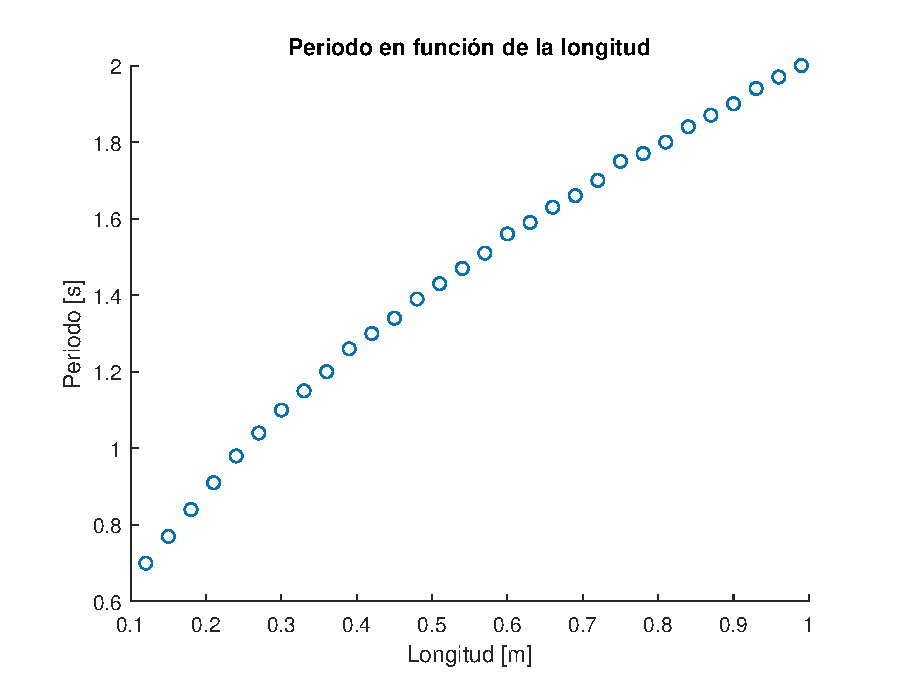
\includegraphics[scale=1.00]{eps/3.4.1.eps}
\caption{Gráfica del péndulo}
\label{practica34}
\end{figure}

La figura \ref{practica34} sugiere un modelo no lineal, así que se aplicara el
método de logaritmos.

La función tiene la forma general:

\begin{equation}
    y = a x^b
\end{equation}

Aplicando logaritmos a ambos lados de la ecuación, obtenemos:

\begin{equation*}
    \log y = \log a + b \log x
\end{equation*}

Haciendo los siguientes cambios de variables:

\begin{equation*}
    Y' = \log y
\end{equation*}
\begin{equation*}
    A = \log a
\end{equation*}
\begin{equation*}
    B = b
\end{equation*}
\begin{equation*}
    X' = \log x
\end{equation*}

Se obtiene:

\begin{equation*}
    Y' = A + B X'
\end{equation*}

\begin{center}
\begin{tabular}{|c|>{\centering}m{2.8cm}<{\centering}
                  |>{\centering}m{2.8cm}<{\centering}|}
\hline
$i$ & $\log(L_i)$ & $\log(T_i)$ \tabularnewline \hline
  1 &  -      &  -      \tabularnewline \hline
  2 & -1.8971 & -0.2614 \tabularnewline \hline
  3 & -1.7148 & -0.1744 \tabularnewline \hline
  4 & -1.5606 & -0.0943 \tabularnewline \hline
  5 & -1.4271 & -0.0202 \tabularnewline \hline
  6 & -1.3093 &  0.0392 \tabularnewline \hline
  7 & -1.2040 &  0.0953 \tabularnewline \hline
  8 & -1.1087 &  0.1398 \tabularnewline \hline
  9 & -1.0217 &  0.1823 \tabularnewline \hline
 10 & -0.9416 &  0.2311 \tabularnewline \hline
 11 & -0.8675 &  0.2624 \tabularnewline \hline
 12 & -0.7985 &  0.2927 \tabularnewline \hline
 13 & -0.7340 &  0.3293 \tabularnewline \hline
 14 & -0.6733 &  0.3577 \tabularnewline \hline
 15 & -0.6162 &  0.3853 \tabularnewline \hline
 16 & -0.5621 &  0.4121 \tabularnewline \hline
 17 & -0.5108 &  0.4447 \tabularnewline \hline
 18 & -0.4620 &  0.4637 \tabularnewline \hline
 19 & -0.4155 &  0.4886 \tabularnewline \hline
 20 & -0.3711 &  0.5068 \tabularnewline \hline
 21 & -0.3285 &  0.5306 \tabularnewline \hline
 22 & -0.2877 &  0.5596 \tabularnewline \hline
 23 & -0.2485 &  0.5710 \tabularnewline \hline
 24 & -0.2107 &  0.5878 \tabularnewline \hline
 25 & -0.1744 &  0.6098 \tabularnewline \hline
 26 & -0.1393 &  0.6259 \tabularnewline \hline
 27 & -0.1054 &  0.6419 \tabularnewline \hline
 28 & -0.0726 &  0.6627 \tabularnewline \hline
 29 & -0.0408 &  0.6780 \tabularnewline \hline
 30 & -0.0101 &  0.6931 \tabularnewline \hline
\end{tabular}
\end{center}

La gráfica de los datos con el cambio de variable logarítmica pueden verse en la
figura \ref{practica34_2}.

\begin{figure}[!h]
\centering
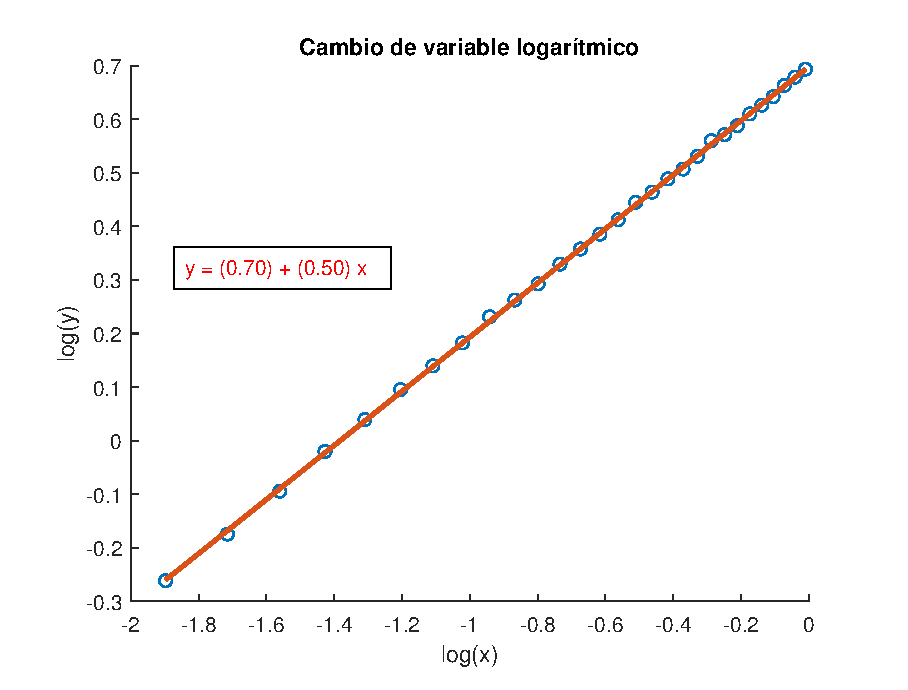
\includegraphics[scale=1.00]{eps/3.4.2.eps}
\caption{Gráfica linealizada por el método de logaritmos}
\label{practica34_2}
\end{figure}

La ecuación de la recta es:

\begin{equation}
    Y = 0.70 + 0.50 x
\end{equation}

A partir de los parámetros de recta $A$ y $B$, calculamos los parámetros $a$ y
$b$, de la curva potencial original:

\begin{equation*}
    a = antilog(A) = antilog(0.70) = 5.0119
\end{equation*}
\begin{equation*}
    b = B = 0.50
\end{equation*}

La ecuación de la curva resultante es:

\begin{equation}
    y = 5.0119 \sqrt{x}
\end{equation}

\subsubsection{Memoria de calculo}

\paragraph{Comandos del programa}
\begin{alltt}
\footnotesize
\input{m/p3_4_2.m}
\normalsize
\end{alltt}

\paragraph{Salida del programa}
\begin{alltt}
\footnotesize
\input{m/o3_4_2.txt}
\normalsize
\end{alltt}

Considerando que el exponente de la ecuación final resultó ser: $0.5$, se
calculará la ecuación por el método del cambio de variable.

La función tiene la forma general:

\begin{equation}
    y = a \sqrt{x}
\end{equation}

Haciendo el siguiente cambio de variable:

\begin{equation*}
    Z = \sqrt{x}
\end{equation*}

\begin{center}
\begin{tabular}{|c|>{\centering}m{2.8cm}<{\centering}
                  |>{\centering}m{2.8cm}<{\centering}|}
\hline
$i$ & $\sqrt{T_i}$ & $L_i$ \tabularnewline \hline
  1 & -      & -      \tabularnewline \hline
  2 & 0.3873 & 0.7700 \tabularnewline \hline
  3 & 0.4243 & 0.8400 \tabularnewline \hline
  4 & 0.4583 & 0.9100 \tabularnewline \hline
  5 & 0.4899 & 0.9800 \tabularnewline \hline
  6 & 0.5196 & 1.0400 \tabularnewline \hline
  7 & 0.5477 & 1.1000 \tabularnewline \hline
  8 & 0.5745 & 1.1500 \tabularnewline \hline
  9 & 0.6000 & 1.2000 \tabularnewline \hline
 10 & 0.6245 & 1.2600 \tabularnewline \hline
 11 & 0.6481 & 1.3000 \tabularnewline \hline
 12 & 0.6708 & 1.3400 \tabularnewline \hline
 13 & 0.6928 & 1.3900 \tabularnewline \hline
 14 & 0.7141 & 1.4300 \tabularnewline \hline
 15 & 0.7348 & 1.4700 \tabularnewline \hline
 16 & 0.7550 & 1.5100 \tabularnewline \hline
 17 & 0.7746 & 1.5600 \tabularnewline \hline
 18 & 0.7937 & 1.5900 \tabularnewline \hline
 19 & 0.8124 & 1.6300 \tabularnewline \hline
 20 & 0.8307 & 1.6600 \tabularnewline \hline
 21 & 0.8485 & 1.7000 \tabularnewline \hline
 22 & 0.8660 & 1.7500 \tabularnewline \hline
 23 & 0.8832 & 1.7700 \tabularnewline \hline
 24 & 0.9000 & 1.8000 \tabularnewline \hline
 25 & 0.9165 & 1.8400 \tabularnewline \hline
 26 & 0.9327 & 1.8700 \tabularnewline \hline
 27 & 0.9487 & 1.9000 \tabularnewline \hline
 28 & 0.9644 & 1.9400 \tabularnewline \hline
 29 & 0.9798 & 1.9700 \tabularnewline \hline
 30 & 0.9950 & 2.0000 \tabularnewline \hline
\end{tabular}
\end{center}

La gráfica de los datos con el cambio de variable puede verse en la figura
\ref{practica34_3}.

\begin{figure}[!h]
\centering
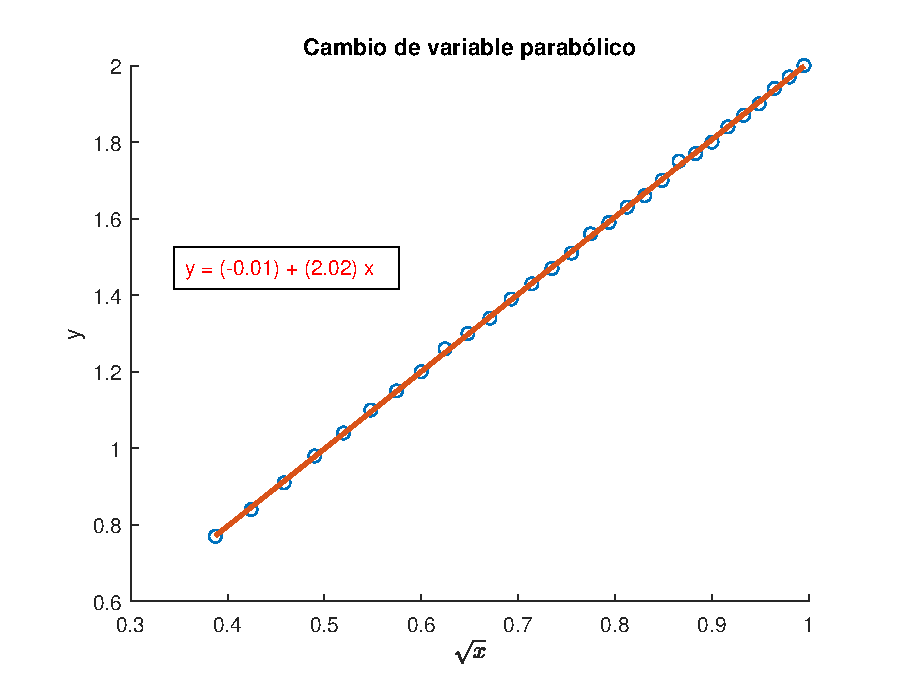
\includegraphics[scale=1.00]{eps/3.4.3.eps}
\caption{Gráfica linealizada por el método de cambio de variable}
\label{practica34_3}
\end{figure}

La ecuación de la recta es:

\begin{equation}
    y = -0.01 + 2.02 Z
\end{equation}

La ecuación de la curva resultante es:

\begin{equation}
    y = -0.01 + 2.02 \sqrt{x}
\end{equation}

\subsubsection{Memoria de calculo}

\paragraph{Comandos del programa}
\begin{alltt}
\footnotesize
\input{m/p3_4_3.m}
\normalsize
\end{alltt}

\paragraph{Salida del programa}
\begin{alltt}
\footnotesize
\input{m/o3_4_3.txt}
\normalsize
\end{alltt}

\end{document}
